\chapter{Specifikacija programske potpore}
		
	\section{Funkcionalni zahtjevi}
			
			% \textbf{\textit{dio 1. revizije}}\\
			
			% \textit{Navesti \textbf{dionike} koji imaju \textbf{interes u ovom sustavu} ili  \textbf{su nositelji odgovornosti}. To su prije svega korisnici, ali i administratori sustava, naručitelji, razvojni tim.}\\
				
			% \textit{Navesti \textbf{aktore} koji izravno \textbf{koriste} ili \textbf{komuniciraju sa sustavom}. Oni mogu imati inicijatorsku ulogu, tj. započinju određene procese u sustavu ili samo sudioničku ulogu, tj. obavljaju određeni posao. Za svakog aktora navesti funkcionalne zahtjeve koji se na njega odnose.}\\
			
			
			\noindent \textbf{Dionici:}
			
			\begin{packed_enum}
				
				\item Nikolina Frid
				\item Andrija Gorup 
				\item Razvojni tim
				\item Korisnici
				\item Administrator
				
			\end{packed_enum}
			
			\noindent \textbf{Aktori i njihovi funkcionalni zahtjevi:}
			
			
			\begin{packed_enum}

				\item  \underbar{korisnik (inicijator) može:}
				
				\begin{packed_enum}
					
					\item pretražiti recept po značajkama
					\item pregledati recept
					\item osvježiti broj porcija, čime će se ažurirati mjerice sastojaka u skladu s navedenim brojem porcija
					\item otvoriti profile registriranih korisnika koji su postavili recept
					
				\end{packed_enum}

				\item  \underbar{Neregistrirani korisnik (inicijator) može:}
				
				\begin{packed_enum}

					\item sve što i korisnik (specijalizacija korisnika)
					\item otvoriti novi korisnički račun za koji je potrebno unjeti korisničko ime koje nije već zauzeto, adresu elektroničke pošte i lozinku računa
					
				\end{packed_enum}

				\item  \underbar{Registrirani korisnik (inicijator) može:}
				
				\begin{packed_enum}
					
					\item sve što i korisnik (specijalizacija korisnika)
					\item ažurirati profil, podaci koje je moguće ažurirati su email, broj telefona i vremenski period u kojima je korisnik dostupan
					\item objaviti recept s obaveznim navođenjem naziva recepta, sastojaka, postupka pripreme i ukupnog trajanja pripreme, mogućnost navođenja dodatnih karakteristika poput oznaka tipa jela i dodavanja slika i videozapisa
					\item ažuriranje već objavljenih recepata
					\item ocijeniti objavu
					\item spremiti recept kako bi im mogli lakše pristupiti kasnije
					\item zapratiti drugog autora (registriranog korisnika), korisnik će dobiti obavijest kada autor objavi novi recept
					\item pregledati vlastiti profil
					\item dodavanje nove oznake poput kategorije ili vrste kuhinje
					\item brisati recepte sa svojeg profila
					\item pisanje komentara na recepte drugih korisnika
					\item slanje poruka u privatnom chatu
					\item pregled poruka privatnih chatova
					
				\end{packed_enum}

				\item  \underbar{Administrator (inicijator) može:}
				\begin{packed_enum}

					\item sve što i korisnik (specijalizacija korisnika)
					\item brisanje korisničkog profila
					\item brisanje recepata
					\item dodati novog administratora
					\item pregled mogućnosti administratora
					\item pristupiti statistikama (npr. najpopularniji recept po broju profila koji su ga spremili, najaktivniji profil s najviše recepata, najpopularniji profil s najčešće spremljenim receptima)
					\item brisanje komentara koji nisu u skladu s pravilima ophođenja na platformi

				\end{packed_enum}
			
				\item  \underbar{Baza podataka (sudionik) može:}
				
				\begin{packed_enum}
					
					\item pohranjuje sve podatke o korisnicima i njihovim ovlastima
					\item pohranjuje sve podatke o receptima
					\item pohranjuje informacije o odnosima među korisnika i recepata
					
				\end{packed_enum}
			\end{packed_enum}
			
			\eject 
			
			
				
			\subsection{Obrasci uporabe}
					
					%Općenita napomena za UC - u .txt skici se kao sudionik često navodi back-end
					%Budući da nije naveden u aktorima, umjesto toga piše baza podataka
					\noindent \underbar{\textbf{UC1 - Pregled recepta}}
					\begin{packed_item}
						
						\item \textbf{Glavni sudionik: }Korisnik
						\item \textbf{Cilj: }Pregledati objavljene recepte
						\item \textbf{Sudionici: }Baza podataka
						\item \textbf{Preduvjet: }-
						\item \textbf{Opis osnovnog tijeka:}
						
						\item[] \begin{packed_enum}
								\item Korisnik odabire recept koji se prikaže
								\end{packed_enum}
					\end{packed_item}
					
					\noindent \underbar{\textbf{UC2 - Pretraživanje recepata}}
					\begin{packed_item}
						
						\item \textbf{Glavni sudionik: }Korisnik
						\item \textbf{Cilj: }Prikazati recepte u skladu s podatcima unesenim u tražilicu
						\item \textbf{Sudionici: }Baza podataka
						\item \textbf{Preduvjet: }-
						\item \textbf{Opis osnovnog tijeka:}
						
						\item[] \begin{packed_enum}
							\item Korisnik odabire pretraživanje recepata
							\item Upisuje ključnu riječ (kategorija, vrsta kuhinje, specifični sastojci)
							\item Baza podataka vraća recepte koji odgovaraju parametrima pretrage
							\item Dobiveni recepti prikazuju se u aplikaciji
						\end{packed_enum}
						\item \textbf{Opis mogućih odstupanja:}
						\item[] \begin{packed_enum}
							\item[3.a] U bazi podataka ne nalazi se niti jedan recept koji odgovara unesenim parametrima
							\begin{packed_enum}
								\item[1.] Sustav korisniku prikazuje poruku da trenutno nema recepata koji odgovaraju njegovom unosu
							\end{packed_enum}
						\end{packed_enum}
					\end{packed_item}
					
					\noindent \underbar{\textbf{UC3 - Registriranje novog korisnika}}
					\begin{packed_item}
						
						\item \textbf{Glavni sudionik: }Neregistrirani korisnik
						\item \textbf{Cilj: }Stvaranje novog korisničkog računa
						\item \textbf{Sudionici: }Baza podataka
						\item \textbf{Preduvjet: }-
						\item \textbf{Opis osnovnog tijeka:}
						%Ovo će možda trebati mijenjati u budućnosti kada budemo radili implementaciju
						\item[] \begin{packed_enum}
							\item Neregistrirani korisnik odabire opciju za registraciju
							\item Unosi potrebne podatke (korisničko ime, adresu elektroničke pošte i lozinku)
							\item Baza podataka provjerava jesu li korisničko ime ili e-mail adresa već zauzeti
							\item Ako su korisničko ime i e-mail adresa slobodni, novog registriranog korisnika se upisuje u bazu
							\item Učitava se naslovna stranica
						\end{packed_enum}
						\item \textbf{Opis mogućih odstupanja:}
						\item[] \begin{packed_enum}
							\item[3.a] Korisničko ime ili adresa elektroničke pošte već su zauzeti
							\begin{packed_enum}
								\item[1.] Korisnik dobiva poruku da su korisničko ime ili e-mail adresa već korišteni
								\item[2.] Korisnika se traži ponovni upis podataka
							\end{packed_enum}
						\end{packed_enum}
					\end{packed_item}
					
					\noindent \underbar{\textbf{UC4 - Prikazivanje tuđeg korisničkog profila}}
					\begin{packed_item}
						
						\item \textbf{Glavni sudionik: }Korisnik
						\item \textbf{Cilj: }Pregled profila drugog registriranog korisnika
						\item \textbf{Sudionici: }Baza podataka
						\item \textbf{Preduvjet: }-
						\item \textbf{Opis osnovnog tijeka:}
						
						\item[] \begin{packed_enum}
							\item Korisnik odabire ikonu autora neke objave
							\item Korisniku se prikazuje profil autora
						\end{packed_enum}
						\item \textbf{Opis mogućih odstupanja:}
						\item[] \begin{packed_enum}
							\item[1.a] Korisnik koristi tražilicu kako bi našao profil koji želi pregledati
							%Što ako koristi tražilicu i nema ničega? Je li to odstupanje na odstupanje? Pitati demosa/asistenta?
							\item[] \begin{packed_enum}
								\item[1.] Korisnik odabire jedan od profila dobivenih pretragom
								\item[2.] Korisniku se prikazuje odabrani profil
							\end{packed_enum}
							\item[2.a] Korisnik pregledava profil koji prati
							\item[] \begin{packed_enum}
								\item[1.] Korisnik otvara vlastiti profil
								\item[2.] Odabire opciju za prikaz profila koje prati
								\item[3.] Korisnik odabire jedan od navedenih profila
								\item[4.] Prikazuje se odabrani profil
							\end{packed_enum}
						\end{packed_enum}
					\end{packed_item}

					\noindent \underbar{\textbf{UC5 - Ažuriranje broj porcija}}
					\begin{packed_item}
						
						\item \textbf{Glavni sudionik: }Korisnik
						\item \textbf{Cilj: }Prikazati potrebne sastojke recepta u skladu s potrebnim porcijama jela
						\item \textbf{Sudionici: }Baza podataka
						\item \textbf{Preduvjet: }UC1 (Pregled recepta)
						\item \textbf{Opis osnovnog tijeka:}
						
						\item[] \begin{packed_enum}
							\item Korisnik na prikazanom receptu stiskanjem tipki (+/-) ažurira broj porcija
							\item Prikaz recepta se ažurira s obzirom na broj porcija
						\end{packed_enum}
					\end{packed_item}

					\noindent \underbar{\textbf{UC6 - Prijava}}
					\begin{packed_item}
						
						\item \textbf{Glavni sudionik: }Registrirani korisnik, Administrator
						\item \textbf{Cilj: }Dobivanje pristupa mogućnostima registriranog korisnika
						\item \textbf{Sudionici: }Baza podataka
						\item \textbf{Preduvjet: }UC3 (Registracija)
						\item \textbf{Opis osnovnog tijeka:}
						
						\item[] \begin{packed_enum}
							\item Registrirani korisnik na naslovnoj stranici odabire opciju za prijavu
							\item Korisnik unosi potrebne podatke (e-mail adresu i lozinku)
							\item Baza podataka provjerava je li korisnik registriran
							\item Baza podataka provjerava je li lozinka ispravna
							\item Učitava se naslovna stranica
						\end{packed_enum}
						\item \textbf{Opis mogućih odstupanja:}
						\item[] \begin{packed_enum}
							\item[3.a] Korisnik nije registriran
							\begin{packed_enum}
								\item[1.] Korisnik dobiva poruku da nije registriran
								\item[2.] Korisnika se preusmjerava na obrazac za registraciju
							\end{packed_enum}
							\item[4.a] Lozinka nije ispravna
							\begin{packed_enum}
								\item[1.] Korisnika se traži da upiše ispravnu lozinku
							\end{packed_enum}
						\end{packed_enum}
					\end{packed_item}
					
					\noindent \underbar{\textbf{UC7 - Objava recepta}}
					\begin{packed_item}
						
						\item \textbf{Glavni sudionik: }Registrirani korisnik
						\item \textbf{Cilj: }Objava novog recepta
						\item \textbf{Sudionici: }Baza podataka
						\item \textbf{Preduvjet: }UC6 (Prijava)
						\item \textbf{Opis osnovnog tijeka:}
						
						\item[] \begin{packed_enum}
							\item Korisnik odabire opciju za novu objavu
							\item Korisnik unosi naslov recepta, sastojke, upute za pripremu i vrijeme pripreme te po izboru dodaje i oznake kategorija, slike i videozapise
							\item Baza podataka zapisuje novi recept i moguće nove oznake unesene
							\item Svi pratitelji autora dobivaju obavijest o novom receptu
						\end{packed_enum}
					\end{packed_item}
					
					\noindent \underbar{\textbf{UC8 - Uređivanje objave}}
					\begin{packed_item}
						
						\item \textbf{Glavni sudionik: }Registrirani korisnik
						\item \textbf{Cilj: }Urediti prethodno objavljeni recept
						\item \textbf{Sudionici: }Baza podataka
						\item \textbf{Preduvjet: }UC7 (Objava recepta)
						\item \textbf{Opis osnovnog tijeka:}
						
						\item[] \begin{packed_enum}
							\item Korisnik odabire pregled vlastitog profila
							\item Korisnik odabire objavu koju želi urediti
							\item Odabire opciju za uređivanje
							\item Korisnik uređuje sadržaj recepta
							\item Po završetku odabire opciju za kraj uređivanja
							\item Baza podataka ažurira recept i dodaje moguće nove oznake
						\end{packed_enum}
					\end{packed_item}
					
					\noindent \underbar{\textbf{UC9 - Brisanje objave}}
					\begin{packed_item}
						
						\item \textbf{Glavni sudionik: }Registrirani korisnik
						\item \textbf{Cilj: }Brisanje prethodno objavljenog recepta
						\item \textbf{Sudionici: }Baza podataka
						\item \textbf{Preduvjet: }UC7 (Objava recepta)
						\item \textbf{Opis osnovnog tijeka:}
						
						\item[] \begin{packed_enum}
							\item Korisnik odabire pregled vlastitog profila
							\item Korisnik odabire objavu koju želi obrisati
							\item Korisnik odabire opciju za brisanje
							\item Baza podataka briše odabrani recept
						\end{packed_enum}
					\end{packed_item}
					
					
					
					\noindent \underbar{\textbf{UC10 - Slanje poruke drugom registriranom korisniku}}
					\begin{packed_item}
						
						\item \textbf{Glavni sudionik: }Registrirani korisnik
						\item \textbf{Cilj: }Komunikacija među korisnicima putem poruka
						\item \textbf{Sudionici: }Baza podataka
						\item \textbf{Preduvjet: } UC4 (Prikazivanje tuđeg profila)
						\item \textbf{Opis osnovnog tijeka:}
						
						\item[] \begin{packed_enum}
							\item Korisnik odabire opciju za slanje poruke
							\item Otvara se polje za pisanje poruke
							\item Kada napiše poruku, korisnik odabire opciju za slanje
							\item Poruka se upisuje u bazu podataka u inbox primatelja
						\end{packed_enum}
					\end{packed_item}
					
					\noindent \underbar{\textbf{UC11 - Zaprati korisnika}}
					\begin{packed_item}
						
						\item \textbf{Glavni sudionik: }Registrirani korisnik
						\item \textbf{Cilj: }Praćenje drugog korisnika kako bi dobio obavijesti o novim objavama
						\item \textbf{Sudionici: }Baza podataka
						\item \textbf{Preduvjet: }UC4 (Prikazivanje tuđeg profila)
						\item \textbf{Opis osnovnog tijeka:}
						
						\item[] \begin{packed_enum}
							\item Korisnik odabire opciju za praćenje
							\item Baza podataka ažurira popis praćenih korisnika
						\end{packed_enum}
					\end{packed_item}
					
					\noindent \underbar{\textbf{UC12 - Pozovi korisnika na video poziv}}
					\begin{packed_item}
						%Možda ne bi bilo loše ovo razraditi čak i ako nećemo implementirati
						%Imati ćemo nešto za napisati u poglavlju 6 - Zaključak i budući rad
						%"Potrebno je točno popisati funkcionalnosti koje nisu implementirane u ostvarenoj aplikaciji"
						\item \textbf{Glavni sudionik: }Registrirani korisnik (Pozivatelj)
						\item \textbf{Cilj: }Uspostava komunikacije između dva korisnika putem videopoziva
						\item \textbf{Sudionici: }Registrirani korisnik (Korisnik kojeg se zove)
						\item \textbf{Preduvjet: }UC4 (Prikazivanje tuđeg profila)
						\item \textbf{Opis osnovnog tijeka:}
						
						\item[] \begin{packed_enum}
							\item Pozivatelj odabire opciju za pokretanje videopoziva
							\item Korisnik kojeg se zove dobiva obavijest o pozivu
							\item Korisnik kojeg se zove prihvaća poziv
							\item Korisnici razgovaraju
							\item Jedan od korisnika prekida poziv po završetku razgovora
						\end{packed_enum}
						\item \textbf{Opis mogućih odstupanja:}
						\item[] \begin{packed_enum}
							\item[3.a] Korisnik kojeg se zove odbija pozivi ili se ne javlja
							\begin{packed_enum}
								\item[1.] Pozivatelj dobiva poruku da je korisnik kojeg zove nedostupan
							\end{packed_enum}
						\end{packed_enum}
					\end{packed_item}
					
					\noindent \underbar{\textbf{UC13 - Pregled inboxa}}
					\begin{packed_item}
						
						\item \textbf{Glavni sudionik: }Registrirani korisnik
						\item \textbf{Cilj: }Pregled svih poruka i obavijesti
						\item \textbf{Sudionici: }Baza podataka
						\item \textbf{Preduvjet: }UC6 (Prijava)
						\item \textbf{Opis osnovnog tijeka:}
						
						\item[] \begin{packed_enum}
							\item Korisnik odabire opciju za pregled inboxa
							\item Otvara se stranica s popisom svih poruka i obavijesti
						\end{packed_enum}
					\end{packed_item}
					
					\noindent \underbar{\textbf{UC14 - Odgovaranje na poruku}}
					\begin{packed_item}
						
						\item \textbf{Glavni sudionik: }Registrirani korisnik
						\item \textbf{Cilj: }Poslati odgovor na dobivenu poruku
						\item \textbf{Sudionici: }Baza podataka
						\item \textbf{Preduvjet: }UC13 (Otvaranje inboxa)
						\item \textbf{Opis osnovnog tijeka:}
						
						\item[] \begin{packed_enum}
							\item Korisnik odabire opciju za otvaranje inboxa
							\item Korisnik odabire poruku na koju želi odgovoriti
							\item Odabire opciju za odgovor
							\item Otvara se polje za sastavljanje poruke
							\item Korisnik piše odgovor
							\item Kada je gotov, odabire opciju za slanje
							\item Poruka se upisuje u bazu podataka u inbox primatelja
						\end{packed_enum}
					\end{packed_item}
					
					%Ovo možda razdvojiti na dva UC-a ili ostaviti samo jednu od opcija
					%Pričali smo o ovome ali ne sijećam se koji je na kraju bio zaključak
					\noindent \underbar{\textbf{UC15 - Ocijeni objavu}}
					\begin{packed_item}
						
						\item \textbf{Glavni sudionik: }Registrirani korisnik
						\item \textbf{Cilj: }Ocijeniti recept s ocjenom od 1 do 5
						\item \textbf{Sudionici: }Baza podataka
						\item \textbf{Preduvjet: }UC6 (Prijava)
						\item \textbf{Opis osnovnog tijeka:}
						
						\item[] \begin{packed_enum}
							\item Korisnik otvara recept koji želi ocijeniti
							\item Korisnik odabire ocjenu koju želi dati
							\item U bazi podataka se ažurira ocjena
						\end{packed_enum}
					\end{packed_item}
					
					\noindent \underbar{\textbf{UC16 - Spremi recept}}
					\begin{packed_item}
						
						\item \textbf{Glavni sudionik: }Registrirani korisnik
						\item \textbf{Cilj: }Spremiti recept kako bi ga se kasnije moglo lakše opet pronaći
						\item \textbf{Sudionici: } Baza podataka
						\item \textbf{Preduvjet: } UC6 (Prijava)
						\item \textbf{Opis osnovnog tijeka:}
						
						\item[] \begin{packed_enum}
							\item Korisnik otvara recept koji želi spremiti
							\item Odabire opciju za spremanje recepta
							\item U bazi podataka se ažurira relacija spremanja u odnosu na korisnika i recepta
						\end{packed_enum}
					\end{packed_item}
										
					\noindent \underbar{\textbf{UC17 - Komentiraj objavljeni recept}}
					\begin{packed_item}
						
						\item \textbf{Glavni sudionik: } Registrirani korisnik
						\item \textbf{Cilj: }Ostaviti komentar na nekoj objavi
						\item \textbf{Sudionici: }Baza podataka
						\item \textbf{Preduvjet: }UC6 (Prijava)
						\item \textbf{Opis osnovnog tijeka:}
						
						\item[] \begin{packed_enum}
							\item Korisnik otvara objavljeni recept
							\item Korisnik otvara komentare na objavi
							\item Korisnik odabire opciju za pisanje komentara
							\item Otvara se polje za pisanje komentara
							\item Korisnik piše komentar i zatim odabire opciju za objavu
							\item Komentar se zapisuje u bazu podataka
						\end{packed_enum}
							%Tek mi je ovdje palo na pamet, ali ista stvar vrijedi i za druge UC-ove
							%Treba li dodati opciju za odustajanje od pisanja komentara?
							%To bi onda vjerojatno bilo odstupanje, ali vjerojatno cijela ideja predstavlja previše nepotrebnog filozofiranja
					\end{packed_item}
										
					\noindent \underbar{\textbf{UC18 - Pregled vlastitog profila}}
					\begin{packed_item}
						
						\item \textbf{Glavni sudionik: }Registrirani korisnik
						\item \textbf{Cilj: }Pregledati stanje vlastitog korisničkog profila
						\item \textbf{Sudionici: }Baza podataka
						\item \textbf{Preduvjet: }UC6 (Prijava)
						\item \textbf{Opis osnovnog tijeka:}
						
						\item[] \begin{packed_enum}
							\item Korisnik na početnoj stranici odabire svoju ikonu
							\item Otvara se stranica na kojoj je prikazan korisnikov profil i njegove objave
						\end{packed_enum}
					\end{packed_item}
										
					\noindent \underbar{\textbf{UC19 - Pregled spremljenih recepata}}
					\begin{packed_item}
						
						\item \textbf{Glavni sudionik: }Registrirani korisnik
						\item \textbf{Cilj: }Prikazati korisnikove najdraže recepte
						\item \textbf{Sudionici: }Baza podataka
						\item \textbf{Preduvjet: }UC18 (Pregledavanje vlastitog profila)
						\item \textbf{Opis osnovnog tijeka:}
						
						\item[] \begin{packed_enum}
							\item Korisnik odabire opciju za pregled spremljenih recepata
							\item Odgovarajući recepti dohvaćaju se iz baze i prikazuju korisniku
						\end{packed_enum}
					\end{packed_item}
										
					\noindent \underbar{\textbf{UC20 - Pregled profila koje korisnik prati}}
					\begin{packed_item}
						
						\item \textbf{Glavni sudionik: }Registrirani korisnik
						\item \textbf{Cilj: }Pregled popisa profila koje korisnik prati
						\item \textbf{Sudionici: }Baza podataka
						\item \textbf{Preduvjet: }UC18 (Pregledavanje vlastitog profila)
						\item \textbf{Opis osnovnog tijeka:}
						
						\item[] \begin{packed_enum}
							\item Korisnik odabire opciju za pregled profila koje prati
							\item Odgovarajući profili dohvaćaju se iz baze i prikazuju korisniku
						\end{packed_enum}
						%Možda odstupanje ako ne prati nikog?
					\end{packed_item}
										
					\noindent \underbar{\textbf{UC21 - Pregled osobnih postavki}}
					\begin{packed_item}
						
						\item \textbf{Glavni sudionik: }Registrirani korisnik
						\item \textbf{Cilj: }Pregledavanje postavki korisničkog profila
						\item \textbf{Sudionici: }Baza podataka
						\item \textbf{Preduvjet: }UC18 (Pregledavanje vlastitog profila)
						\item \textbf{Opis osnovnog tijeka:}
						
						\item[] \begin{packed_enum}
							\item Korisnik odabire opciju za pregled postavki profila
							\item Prikazuju se postavke profila
						\end{packed_enum}
					\end{packed_item}
										
					\noindent \underbar{\textbf{UC22 - Brisanje vlastitog profila}}
					\begin{packed_item}
						
						\item \textbf{Glavni sudionik: }Registrirani korisnik
						\item \textbf{Cilj: }Brisanje vlastitog korisničkog profila
						\item \textbf{Sudionici: }Baza podataka
						\item \textbf{Preduvjet: }UC21 (Pregled osobnih postavki)
						\item \textbf{Opis osnovnog tijeka:}
						
						\item[] \begin{packed_enum}
							\item Korisnik odabire opciju za brisanje računa
							\item Profil se briše iz baze podataka, recepti i komentari ostaju, ali piše da ih je objavio obrisani korisnik
						\end{packed_enum}
					\end{packed_item}
										
					\noindent \underbar{\textbf{UC23 - Uređivanje osobnih postavki}}
					\begin{packed_item}
						
						\item \textbf{Glavni sudionik: }Registrirani korisnik
						\item \textbf{Cilj: }Promjena postavki profila
						\item \textbf{Sudionici: }Baza podataka
						\item \textbf{Preduvjet: }UC21 (Pregled osobnih postavki)
						\item \textbf{Opis osnovnog tijeka:}
						
						\item[] \begin{packed_enum}
							\item Korisnik odabire opciju za uređivanje postavki
							\item Korisnik mijenja željene postavke
							\item Postavke se ažuriraju u bazi podataka
						\end{packed_enum}
					\end{packed_item}
										
										
					\noindent \underbar{\textbf{UC24 - Dodavanje novog administratora}}
					\begin{packed_item}
						
						\item \textbf{Glavni sudionik: }Administrator
						\item \textbf{Cilj: }Dodati novog administratora
						\item \textbf{Sudionici: }Baza podataka
						\item \textbf{Preduvjet: }UC6 (Prijava)
						\item \textbf{Opis osnovnog tijeka:}
						
						\item[] \begin{packed_enum}
							\item Administrator odabire opciju stvaranja novog administratora
							\item Upisuje potrebne informacija za kreiranje admina, korisničko ime i lozinka
							\item Baza podataka se ažurira i dodaje novog administratora
						\end{packed_enum}
						\item \textbf{Opis mogućih odstupanja:}
					\end{packed_item}
										
					\noindent \underbar{\textbf{UC25 - Brisanje recepta}}
					\begin{packed_item}
						
						\item \textbf{Glavni sudionik: }Administrator
						\item \textbf{Cilj: }Brisanje recepta koji nije prikladan ili slično
						\item \textbf{Sudionici: }Baza podataka
						\item \textbf{Preduvjet: }UC6 (Prijava)
						\item \textbf{Opis osnovnog tijeka:}
						
						\item[] \begin{packed_enum}
							\item Administrator odabire recept koji želi obrisati
							\item Odabire opciju za brisanje
							\item Recept, njegovi komentari i ostali povezani podatci brišu se iz baze podataka
						\end{packed_enum}
					\end{packed_item}
										
					\noindent \underbar{\textbf{UC26 - Brisanje korisnika}}
					\begin{packed_item}
						
						\item \textbf{Glavni sudionik: }Administrator
						\item \textbf{Cilj: }Brisanje korisničkog profila
						\item \textbf{Sudionici: }Baza podataka
						\item \textbf{Preduvjet: }UC6 (Prijava)
						\item \textbf{Opis osnovnog tijeka:}
						
						\item[] \begin{packed_enum}
							\item Administrator odabire profil koji želi obrisati
							\item Odabire opciju za brisanje
							\item Korisniku se elektroničkom poštom šalje obavijest o brisanju
							\item Profil se briše iz baze podataka
						\end{packed_enum}
					\end{packed_item}
										
					\noindent \underbar{\textbf{UC27 - Pregled mogućnosti administratora}}
					\begin{packed_item}
						
						\item \textbf{Glavni sudionik: }Administrator
						\item \textbf{Cilj: }Pristup svim administratorskim mogućnostima
						\item \textbf{Sudionici: }Baza podataka
						\item \textbf{Preduvjet: }UC6 (Prijava)
						\item \textbf{Opis osnovnog tijeka:}
						
						\item[] \begin{packed_enum}
							\item Administrator odabire opciju za prikaz administratorskih mogućnosti
							\item Prikazuje se pregled i mogućnosti za upravljanje bazom podataka
						\end{packed_enum}
					\end{packed_item}
					
					

					\noindent \underbar{\textbf{UC28 - Brisanje komentara s recepata}}
					\begin{packed_item}
						
						\item \textbf{Glavni sudionik: }Administrator
						\item \textbf{Cilj: }Obrisati neprimjerene komentare s objava
						\item \textbf{Sudionici: }Baza podataka
						\item \textbf{Preduvjet: }UC6 (Prijava)
						\item \textbf{Opis osnovnog tijeka:}
						
						\item[] \begin{packed_enum}
							\item Administrator odabire komentar koji želi obrisati
							\item Odabire opciju za brisanje
							\item Korisniku se elektroničkom poštom šalje obavijest o brisanju njegovog napisanog komentara
							\item Komentar se briše iz baze podataka
						\end{packed_enum}
					\end{packed_item}

					\noindent \underbar{\textbf{UC29 - Pregled statistike platforme}}
					\begin{packed_item}
						
						\item \textbf{Glavni sudionik: }Administrator
						\item \textbf{Cilj: }Dobiti uvid u najbolji recept (po ocjeni), najaktivnije korisnike (po broju objava) i najpopularniji recept (po broju spremanja)
						\item \textbf{Sudionici: }Baza podataka
						\item \textbf{Preduvjet: }UC27 (Pregled mogućnosti administratora)
						\item \textbf{Opis osnovnog tijeka:}
						
						\item[] \begin{packed_enum}
							\item Administrator odabire opciju za pregled statistika
							\item Prikazuje se pregled
						\end{packed_enum}
					\end{packed_item}
					%Nisam siguran na što se točno misli pod UC 31 i 32 (u obrasci_uporabe.txt), ali bilo bi ih dobro imati iz istog razloga kao i UC11 (videopoziv)
				
					
				\subsubsection{Dijagrami obrazaca uporabe}
					
					% \textit{Prikazati odnos aktora i obrazaca uporabe odgovarajućim UML dijagramom. Nije nužno nacrtati sve na jednom dijagramu. Modelirati po razinama apstrakcije i skupovima srodnih funkcionalnosti.}
					\begin{figure}[H]
						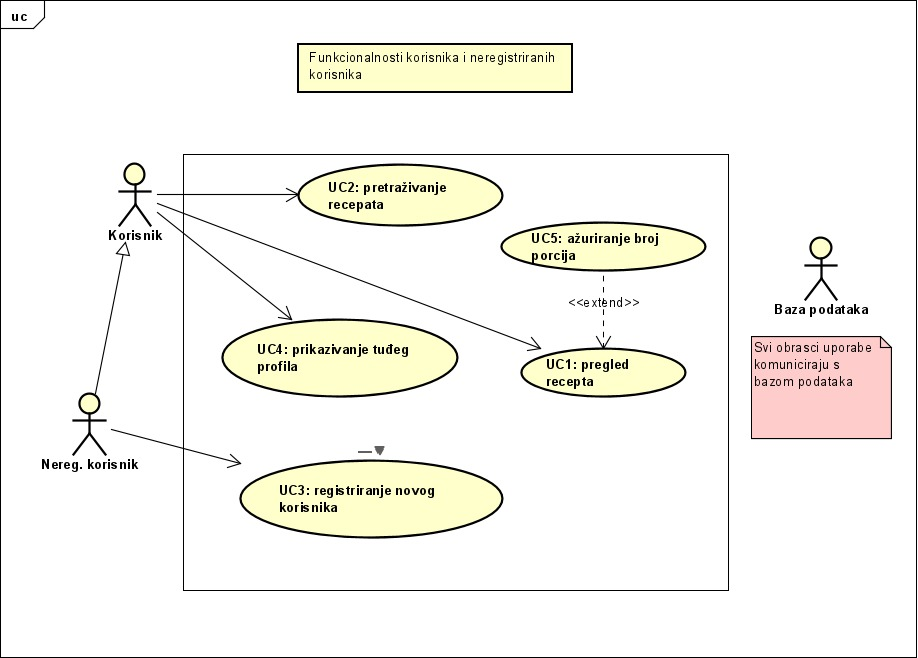
\includegraphics[scale=0.4]{slike/UC_nereg.jpeg} %veličina slike u odnosu na originalnu datoteku i pozicija slike
						\centering
						\caption{Dijagram obrasca uporabe, funkcionalnost korisnika i neregistriranog korisnika}
						\label{fig:UC_diagram1}
					\end{figure}

					\begin{figure}[H]
						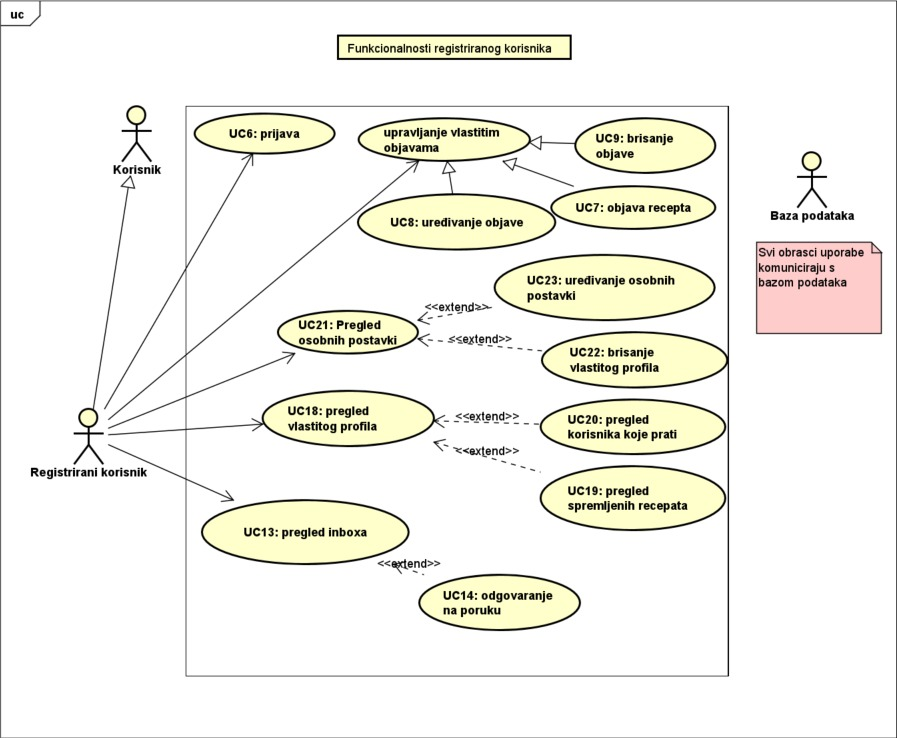
\includegraphics[scale=0.5]{slike/UC_reg.jpeg} %veličina slike u odnosu na originalnu datoteku i pozicija slike
						\centering
						\caption{Dijagram obrasca uporabe, funkcionalnost registriranog korisnika}
						\label{fig:UC_diagram2}
					\end{figure}

					\begin{figure}[H]
						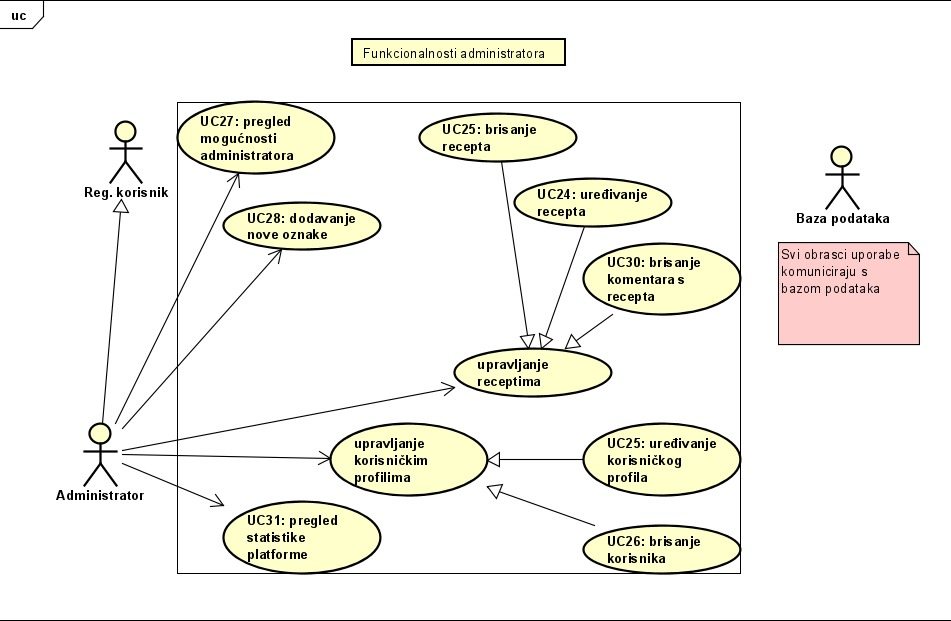
\includegraphics[scale=0.5]{slike/UC_admin.jpeg} %veličina slike u odnosu na originalnu datoteku i pozicija slike
						\centering
						\caption{Dijagram obrasca uporabe, funkcionalnost administratora}
						\label{fig:UC_diagram3}
					\end{figure}
				\eject		
				
			\subsection{Sekvencijski dijagrami}
				
			\begin{figure}[H]
				\textbf{Obrazac uporabe UC3 - Registriranje novog korisnika}\\

				Neregistrirani korisnik šalje zahtjev za registraciju te mu web-aplikacija šalje odgovor formom za registraciju. Dokle god web-aplikacija u bazi podataka provjerom dobije odgovor da su email ili lozinka zauzeti korisnik dobiva poruku o zauzetosti emaila ili lozinke te ponovnu formu za upis podataka. Nakon unosa kod kojeg su email i username dostupni korisnikove informacije se zapisuju u bazu podataka. Korisnik dobiva poruku o uspješnoj registraciji.
				\begin{center}
					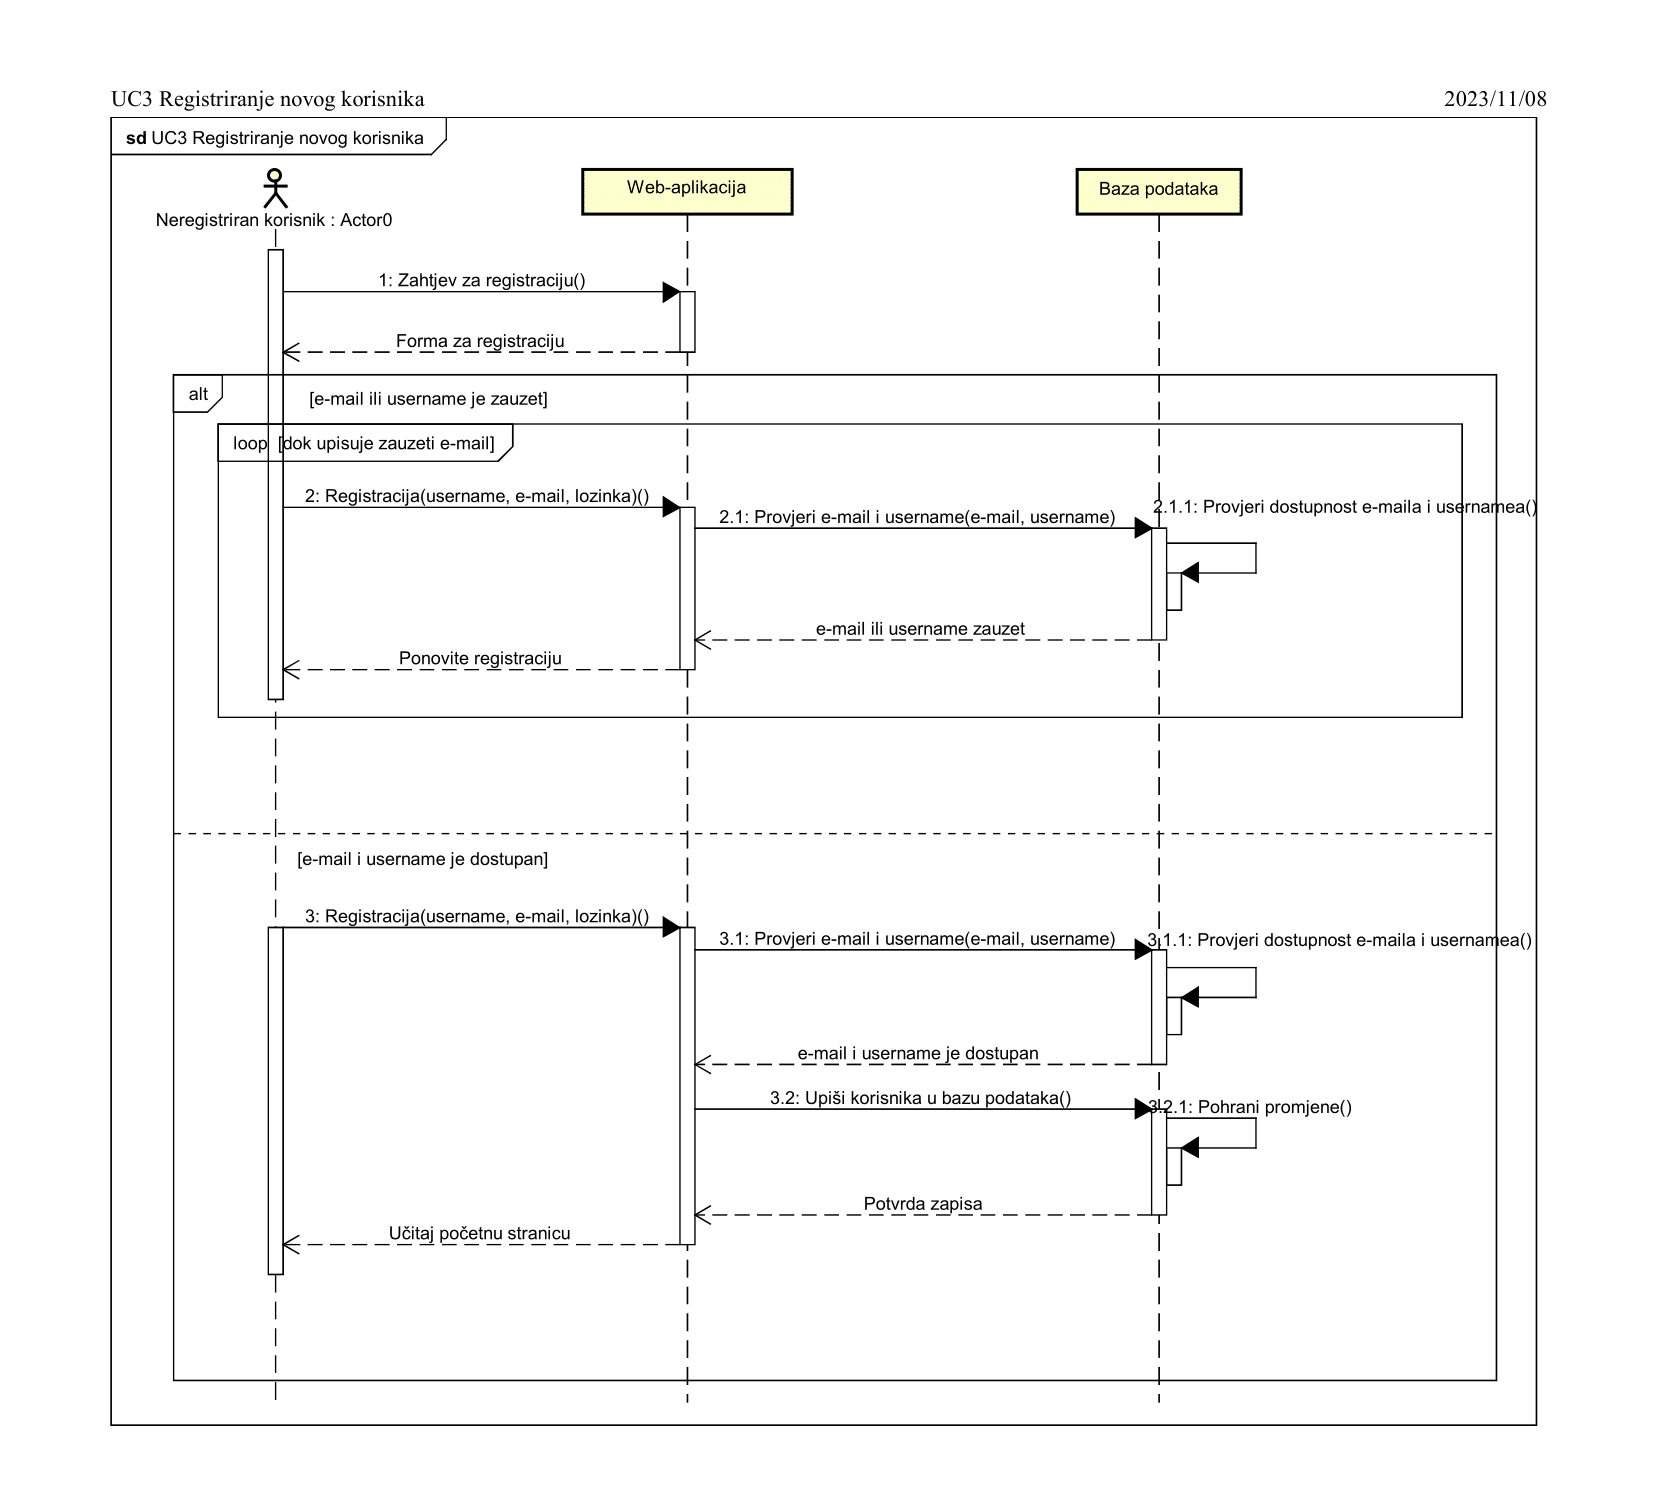
\includegraphics[scale = 0.8]{slike/SEK_UC3_Registriranje_novog_korisnika.png}
					\caption{Sekvencijski dijagram za UC3}
					\label{fig:Sek_UC3}
				\end{center}
			\end{figure}

			\begin{figure}[H]
				\textbf{Obrazac uporabe UC7 - Objava recepta}\\

				Registrirani korisnik šalje zahtjev za objavu recepte, a web-aplikacija mu odgovara formom za unos recepta. Registrirani korisnik unosi podatke o receptu: naslov, sastojci, priprema, vrijeme, kategorije, slike, video. Novonastali recept se zatim sprema u bazu podataka i web-aplikacija dobiva potvrdu o spremljenim podacima. Nakon potvrde web-aplikacija bazi podataka šalje zahtjev sa svim korisnicima koji su pratitelji autora objavljenog recepta te im svima šalje obavijest o novoj objavi.
				\begin{center}
					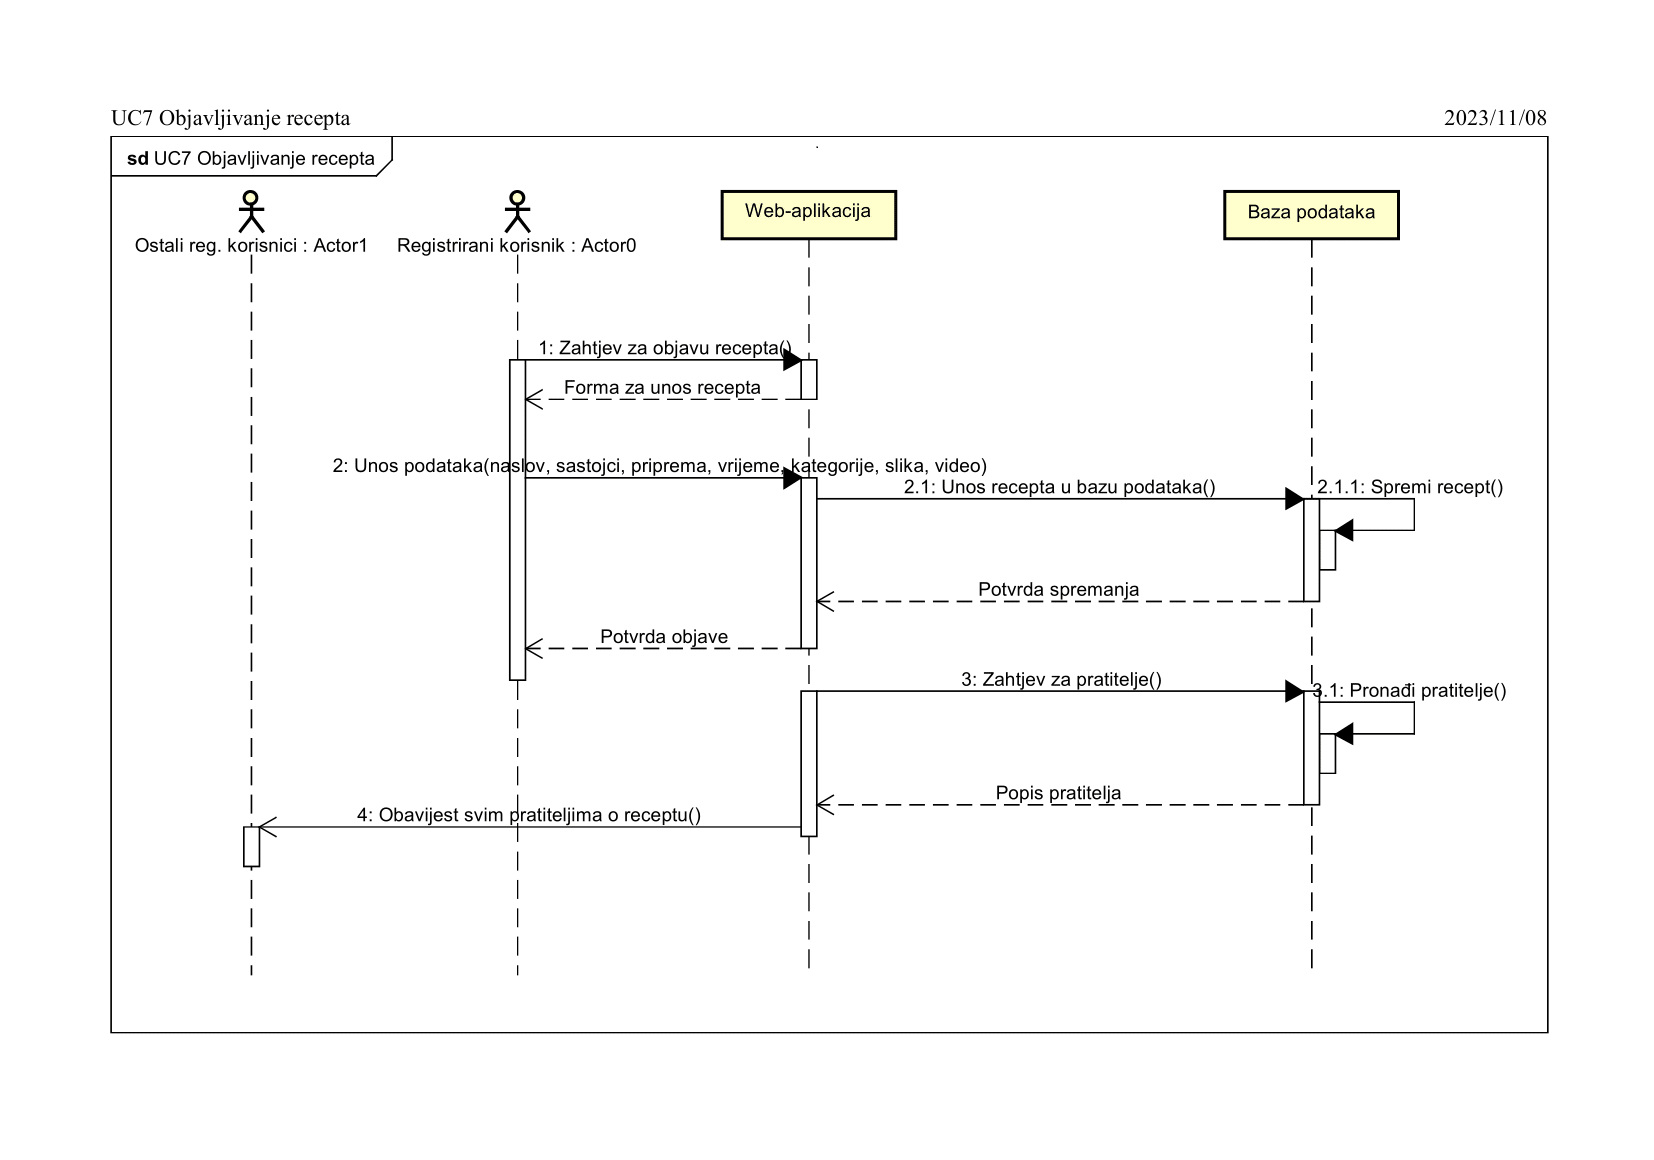
\includegraphics[scale = 0.8]{slike/SEK_UC7_Objavljivanje_recepta.png}
					\caption{Sekvencijski dijagram za UC7}
					\label{fig:Sek_UC7}							
				\end{center}
			\end{figure}

			\begin{figure}[H]
				\textbf{Obrazac uporabe UC18 - Pregled vlastitog profila}\\

				Registrirani korisnik šalje zahtjev za prikaz svog profila i web aplikaciju mu prikazuje sve informacije dobivene iz baze podataka. Nakon toga korisnik može zatražiti popis svih korisnika koji ga prate (UC20 Pregled profila koje korisnik prati), a web-aplikaciju bi mu odgovorila popisom korisnika koju bi dobila slanjem zahtjeva bazi podataka.
				Korisnik može odabrati i opciju pregledavanja spremljenih recepata (UC19 Pregledavanje spremljenih recepata) koji se prikazuju tako što web-aplikacija dobiva popis spremljenih recepata iz baze podataka.
				\begin{center}
					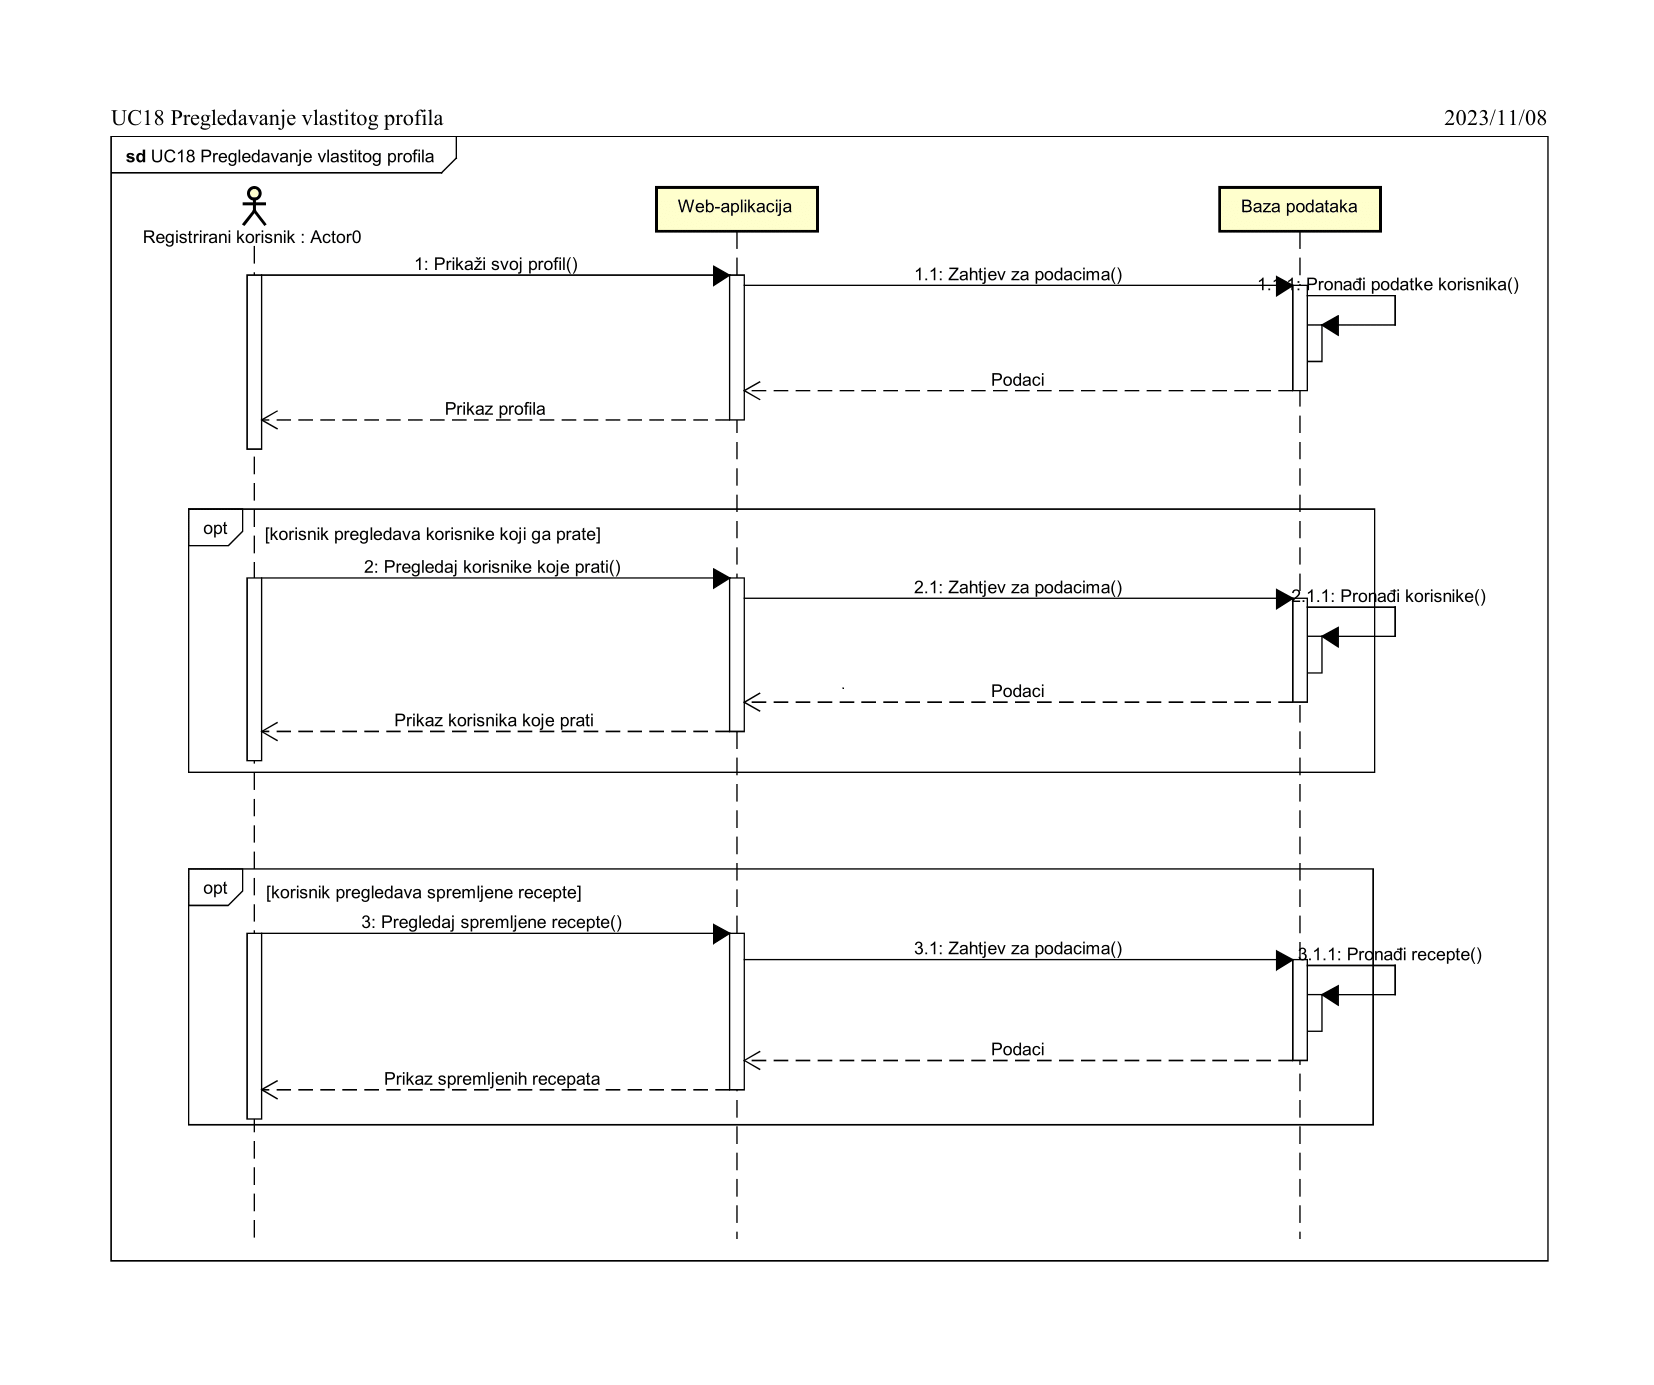
\includegraphics[scale = 0.8]{slike/SEK_UC18_Pregledavanje_vlastitog_profila.png}
					\caption{Sekvencijski dijagram za UC18}
					\label{fig:Sek_UC18}
				\end{center}
			\end{figure}

			\begin{figure}[H]
				\textbf{Obrazac uporabe UC21 - Pregled osobnih postavki}\\

				Registrirani korisnik šalje zahtjev za pregled osobnih postavki. Web-aplikacija prihvaća zahtjev i pošalje upit bazi podataka koja šalje sve podatke korisnika koje može ažurirati/brisati. Korisnik može odabrati opciju uređivanja profila (UC23 Uređivanje osobnih postavki), a web-aplikacija mu šalje formu za uređivanje postavki. Nakon što korisnik upiše promjene, potvrda promjena se šalje web-aplikaciji koja prosljeđuje podatke bazi podataka koja za tog korisnika ažurira promjene. Druga opcija koju korisnik može odabrati je brisanje profila (UC22 Brisanje vlastitog profila). Korisnik šalje zahtjev za brisanje profila web-aplikaciji koja prosljeđuje podatke korisnika bazi podataka koja ga na kraju briše.
				\begin{center}
					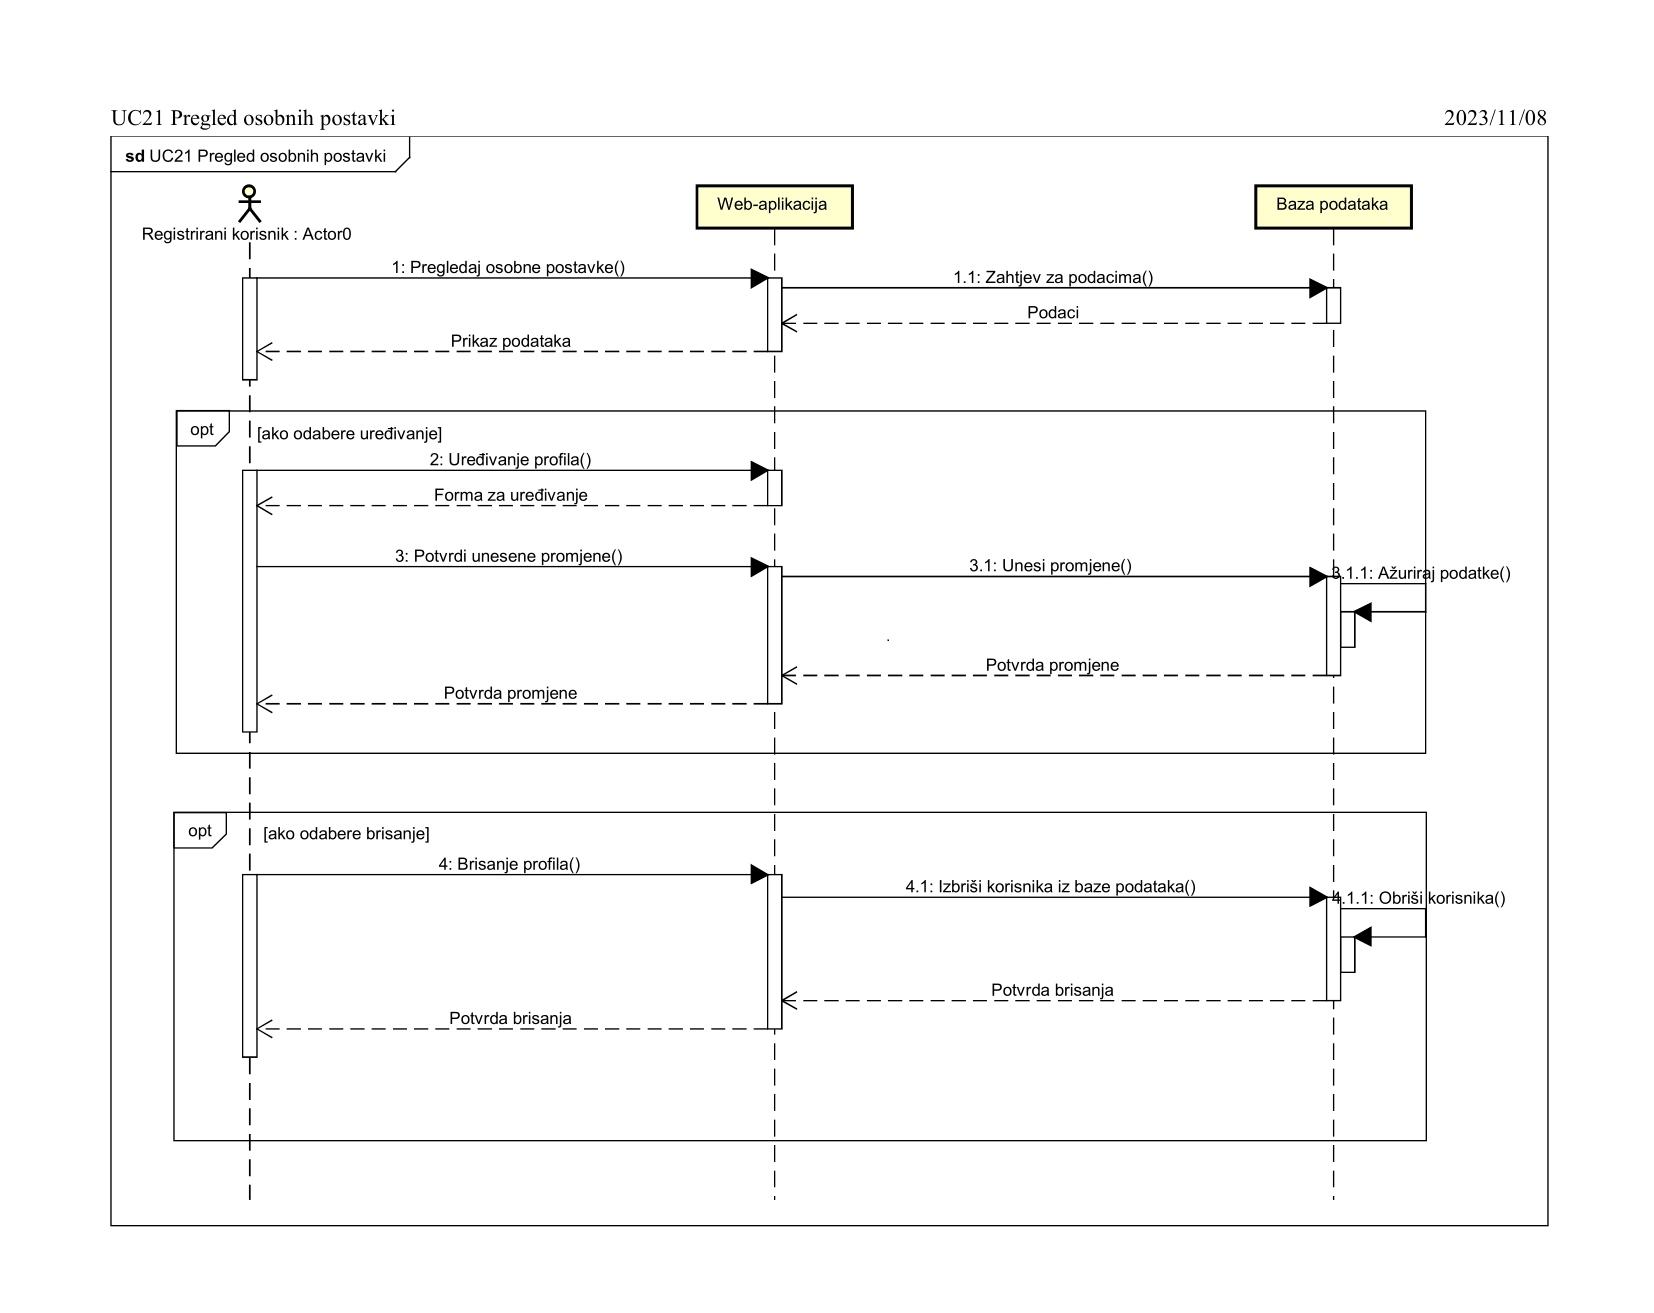
\includegraphics[scale = 0.8]{slike/SEK_UC21_Pregled_osobnih_postavki.png}
					\caption{Sekvencijski dijagram za UC21}
					\label{fig:Sek_UC21}
				\end{center}
			\end{figure}
				
			\eject
	
		\section{Ostali zahtjevi}
			 
			 \begin{packed_item}
			 	\item Aplikaciji se pristupa s pomoću internetskog preglednika korištenjem HTTPS protokola
			 	\item Aplikaciji treba moći pristupiti više korisnika istovremeno
			 	\item Korisničko sučelje mora biti intuitivno i jednostavno za korištenje
			 	\item Dizajn korisničkog sučelja mora biti responzivan kako bi se aplikaciji moglo pristupiti i s mobilnih uređaja
			 	\item Sustav mora biti otporan na greške uzrokovane neispravnim korištenjem korisničkog sučelja
			 	\item Postupak prijave korisnika mora biti siguran, a lozinke ne smiju biti pohranjene kao otvoreni tekst
			 	\item Baza podataka mora sadržavati odgovarajuće indekse kako bi pristup podatcima bio brz
			 	\item Baza podataka mora biti odvojena od ostatka sustava, ne smije joj se moći pristupiti izravno, već samo preko back-enda aplikacije
			 	\item Korisničko sučelje i baza podataka moraju podržavati dijakritičke znakove
			 	\item Pri implementaciji moraju biti korištena načela objektno-orijentiranog programiranja
			 	\item Razvojna verzija aplikacije mora biti u potpunosti odvojena od produkcijske kako rad na nadogradnjama ne bi utjecao na postojeće funkcionalnosti
			 	
			 \end{packed_item}
			 \eject
			 
			 
			 
	